\documentclass[border=4pt]{standalone}
\usepackage[T1]{fontenc}
\usepackage{helvet}
\renewcommand{\familydefault}{\sfdefault}
\usepackage{graphicx}
\usepackage{caption}
\usepackage{amsmath}
\captionsetup{font={sf,footnotesize},labelfont={sf,bf,footnotesize},justification=justified,singlelinecheck=false}
\begin{document}
\setcounter{figure}{4}
\begin{minipage}{7.20in}
\centering
\begin{figure}[htbp]
    \centering
    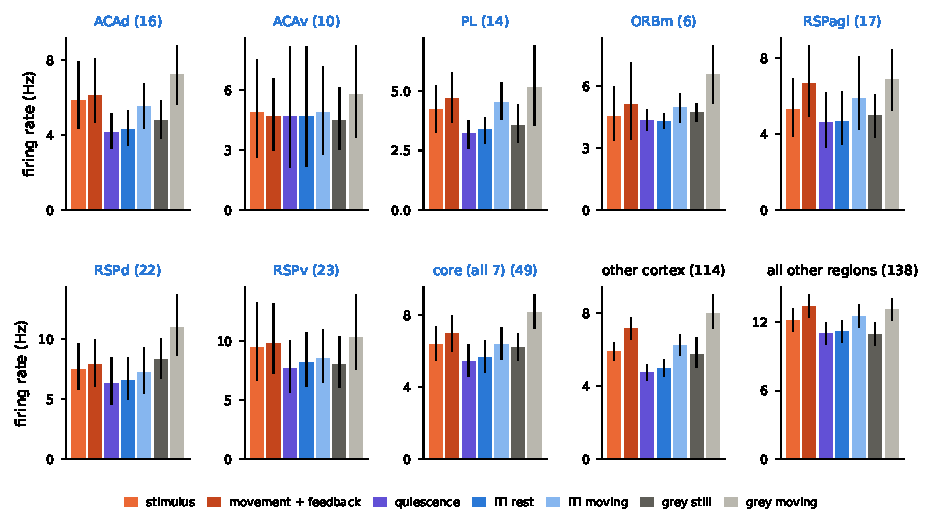
\includegraphics[width=\linewidth]{fig5_windows_panels.pdf}
    \caption{Session-averaged firing rate in seven behavioural windows for each region of the conservative DMN core, the core pooled, all other cortex and all other recorded regions (bars, left to right as in the legend): stimulus (0--0.15 s after onset), movement + feedback (movement onset $-$0.15--0 s, 0--0.15 s and feedback 0--0.3 s; the task windows of Fig. 4), quiescence (still bins from trial start to 0.1 s before the stimulus: engaged, waiting, not moving), ITI rest (still bins between the end of a trial and the start of the next), ITI moving (moving bins in the same gaps), and the grey screen still and moving. Mean over mice of the neuron-averaged rate, 95\% bootstrap CI over mice (number of mice in brackets); 58,417 neurons with $\geq$0.5 Hz, 426 sessions, 138 mice.}
    \label{fig:grey_windows}
\end{figure}
\end{minipage}
\end{document}
